\subsection{The CKM matrix and Unitarity Triangle}
\label{sec:ckm}

The \ckm matrix is defined as:
\begin{equation}
  \VCKM = \left(V_{uL}^{\phantom{\dagger}} V_{dL}^\dagger\right) =
  \begin{pmatrix}
    \V{ud} & \V{us} & \V{ub} \\
    \V{cd} & \V{cs} & \V{cb} \\
    \V{td} & \V{ts} & \V{tb} \\
  \end{pmatrix},
\end{equation}
where each $|V_{ij}|$ parameterizes the probability of an up-type quark, of generation $i$,
transitioning to down-type quark, $j$, in a weak interaction.
In the \sm, it is assumed that the total charged current couplings of up- to down-type quarks is the
same as down- to up-type.
This means that the \ckm matrix is unitary, $\VCKMconj\VCKM = \mathds{1}$, and therefore it contains
only four physical parameters: three angles ($\theta_{12}$, $\theta_{13}$ and $\theta_{23}$) and one
complex phase ($\delta$).
In fact, the observation of \CPV in kaon mixing~\cite{Christenson:1964fg}
led to the prediction of a third generation before
its discovery, precisely because a $3\times3$ matrix is the smallest necessary for a phase to enter
a unitary matrix.

%preferentially
%hierarchichal
%arbiatry

%The CKM matrix is the source of all flavour violation in the SM.
%In the SM, it is assumed that the total charged current couplings of up- to down-type quarks is the
%same as down- to up-type.
%This means that the CKM matrix is unitary, $V^\dagger V = \mathbb{1}$, and therefore it contains
%four physical parameters: three angles ($\theta_{12}$, $\theta_{13}$ and $\theta_{23}$) and one
%complex phase ($\delta$).

%\begin{equation}
  %\VCKM =
  %\begin{pmatrix}
    %\cxx{12}\cxx{13} & \sxx{12}\cxx{13} & \sxx{13}e^{-i\delta} \\
    %-\sxx{12}\cxx{23}-\cxx{12}\sxx{23}\sxx{13}e^{i\delta} &
    %\cxx{12}\cxx{23}-\sxx{12}\sxx{23}\sxx{13}e^{i\delta} & \sxx{23}\cxx{13} \\
    %\sxx{12}\sxx{23}-\cxx{12}\cxx{23}\sxx{13}e^{i\delta} &
    %-\cxx{12}\sxx{23}-\sxx{12}\cxx{23}\sxx{13}e^{i\delta} & \cxx{23}\cxx{13} \\
  %\end{pmatrix}
%\end{equation}

There are many ways of representing the \ckm matrix.
One way is as a product of three rotation
matrices, one of which contains the complex phase, this is known as the \emph{standard}
parameterization:
\begin{equation}
  \VCKM =
  \begin{pmatrix}
    \cxx{12}\cxx{13} & \sxx{12}\cxx{13} & \sxx{13}e^{-i\delta} \\
    -\sxx{12}\cxx{23}-\cxx{12}\sxx{23}\sxx{13}e^{i\delta} &
    \cxx{12}\cxx{23}-\sxx{12}\sxx{23}\sxx{13}e^{i\delta} & \sxx{23}\cxx{13} \\
    \sxx{12}\sxx{23}-\cxx{12}\cxx{23}\sxx{13}e^{i\delta} &
    -\cxx{12}\sxx{23}-\sxx{12}\cxx{23}\sxx{13}e^{i\delta} & \cxx{23}\cxx{13} \\
  \end{pmatrix},
\end{equation}
where $\sxx{ij}$ and $\cxx{ij}$ denote $\sin\theta_{ij}$ and $\cos\theta_{ij}$, respectively.
A convenient simplification is the \emph{Wolfenstein} parameterization, which is obtained by
defining
\begin{align}
  \sin\theta_{12}&=\lambda, \nonumber\\
  \sin\theta_{23}&=A\lambda^2, \nonumber\\
  \intertext{and}
  e^{-i\delta}\sin\theta_{13} &= A\lambda^3(\rho-i\eta),
\end{align}
which results in
\begin{align}
  \VCKM\simeq
  \begin{pmatrix}
      %1-\tfrac12\lambda & \lambda & A\lambda^3(\rho-i\eta+\tfrac{i}2\eta\lambda^2) \\
      %-\lambda & 1-\lambda^2-i\eta A^2\lambda^4 & A\lambda^2(1+i\eta\lambda^2) \\
      %A\lambda^3(1-\rho-i\eta) & -A\lambda^2 & 1 \\
    1-\tfrac12\lambda & \lambda & A\lambda^3\big(\rho-i\eta\big) \\
    -\lambda & 1-\lambda^2 & A\lambda^2 \\
    A\lambda^3\big(1-\rho-i\eta\big) & -A\lambda^2 & 1 \\
  \end{pmatrix}.
  \label{eq:th:wolfenstein}
\end{align}
The values of the Wolfenstein parameters $A$ and $\lambda$ are:
\begin{spacing}{.8}
%{%
  %\setlength{\belowdisplayskip}{4pt}%
  %\setlength{\abovedisplayskip}{4pt}%
  \begin{align*}
  %\lambda &= 0.22537\pm0.00061, \nonumber\\\intertext{cat} A&=0.814\,^{+0.023}_{-0.024}.
    \lambda &= 0.22537\pm0.00061,
    \intertext{and}
    A&=0.814\,^{+0.023}_{-0.024}.
  \end{align*}
\end{spacing}
%}
Since $A\neq0$ and $\lambda\neq0$, it is clear that \VCKM is not diagonal, and therefore
flavour-changing currents are allowed in the \sm.
However,
it is most probable that a weak interaction is intra-generational, meaning that
the \ckm matrix exhibits a strongly hierarchic structure.
%However, the diagonal elements are close to unity and the CKM matrix exhibits a strong
%hierarchical structure, such that it is most probable that weak currents do not violate flavour.
%for which there is no explaination in the SM.


It has been asserted that the \ckm matrix is unitary, and therefore a
unitarity condition can be expressed as
$\Vconj{\alpha\beta}\V{\beta\gamma}=\delta_{\alpha\gamma}$.
%$V_{\alpha\beta}^{\phantom{\dagger}}V_{\beta\gamma}^* = \delta_{\alpha\gamma}$
%\begin{equation}
  %V_{\alpha\beta}^{\phantom{\dagger}}V_{\beta\gamma}^* = \delta_{\alpha\gamma},
  %\boldsymbol{V}_{ij}\boldsymbol{V}_{jk}^\dagger = \delta_{ik}.
  %\sum_{i=1}^3\left|V_{ij}\right|^2 = 1
  %\sum_{i=1}^3\left(V_{ij}^*V_{jk}\right) = \mathbb{1},
  %\label{eq:th:unitarity}
%\end{equation}
When $\delta_{\alpha\gamma}=0$, this condition gives six equations of the form:
\begin{align}
  %\sum_{i=1}^3V_{ij}^*V_{ki} &= 0 && \sum_{i=1}^3V_{ji}^*V_{ik} =0, & j&\neq k;
  \phantom{\beta\neq\gamma}
  &&\sum_{\beta=1}^3V_{\alpha\beta}^*V_{\beta\gamma}^{\phantom{*}} = 0,
  &&\sum_{\beta=1}^3V_{\alpha\beta}^{\phantom{*}}V_{\beta\gamma}^*=0,
  &&\alpha\neq\gamma;
  \label{eq:th:offdiag}
\end{align}
each mapping a closed \replaced{triangle}{triangles} on the complex plane.
Two of these triangles have all sides of similar length
%One of these triangles, which has sides of similar length
$\big(\mathcal{O}(\lambda^3)\big)$,
one of these is
is known as \emph{the} \ut and is defined by
%Taking the equations of the triangles in Eq.~\ref{eq:th:unitarity} where all sides have length of
%$\mathcal{O}(\lambda^3)$ leaves two triangles, one of which is:
\begin{equation}
  %\V{ud}\Vconj{ub} + \V{cd}\Vconj{cb} + \V{td}\Vconj{tb} = 0.
  1 + \frac{\V{ud}\Vconj{ub}}{\V{cd}\Vconj{cb}} + \frac{\V{td}\Vconj{tb}}{\V{cd}\Vconj{cb}} = 0,
  \label{eq:th:ut}
\end{equation}
where the length of the base has been normalized to unity.
The apex of the \ut is at
\begin{align}
  %\bar\rho+i\bar\eta = (1-\tfrac12\lambda^2)(\rho+i\eta)
  \xbar\rho+i\xbar\eta &= \big(1-\tfrac12\lambda^2\big)\big(\rho+i\eta\big)
  \nonumber\\
  &=\frac{\V{ud}\Vconj{ub}}{\V{cd}\Vconj{cb}},
\end{align}
%If divided through by $\V{cd}\Vconj{cb}$, then Eq.~\ref{eq:th:ut} can be mapped onto the complex
%plane, where the apex is at $\bar\rho+i\bar\eta = (1-\tfrac12\lambda^2)(\rho+i\eta)$.
%and the angles are
and forms the angles
\begin{align}
  \alpha &= \arg\left(-\frac{\V{td}\Vconj{tb}}{\V{ud}\Vconj{ub}}\right), &
  \beta  &= \arg\left(-\frac{\V{cd}\Vconj{cb}}{\V{td}\Vconj{tb}}\right), &
  \gamma &= \arg\left(-\frac{\V{ud}\Vconj{ub}}{\V{cd}\Vconj{cb}}\right).
  %\alpha &=    \arg\left(-\frac{\V{td}\Vconj{tb}}{\V{ud}\Vconj{ub}}\right), \nonumber\\
  %\beta  &=\pi-\arg\left( \frac{\V{td}\Vconj{tb}}{\V{cd}\Vconj{cb}}\right), \nonumber\\
  %%& &\mathrm{and}
  %\gamma &=    \arg\left( \frac{\V{ud}\Vconj{ub}}{\V{cd}\Vconj{cb}}\right).
  \label{eq:ut:angles}
\end{align}
which define phase differences between edges.
Figure~\ref{fig:th:ut} depicts a schematic diagram of the \ut.
%are phases between CKM matrix elements.
%This triangle is depicted in \Fig{fig:th:ut}.
%, is simply a graphical representation of the CKM matrix.
%Measurements of CKM matrix elements constrain the angles, side lengths and apex of the UT, these
%constraints are also shown in Fig.~\ref{fig:th:ut}.

\begin{figure}
  \begin{center}
      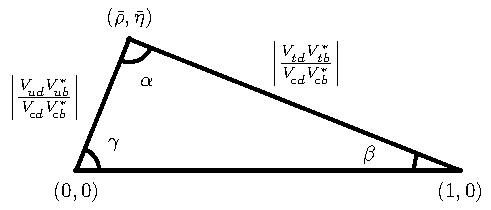
\includegraphics[scale=1.1]{diagram_ut}
  \end{center}
  \caption[Schematic diagram of the Unitarity Triangle]
  {
    Schematic diagram of the Unitarity triangle given in Eq.~\protect\ref{eq:th:ut} on the complex
    plane, where the base has been normalized to unit length.
    The angles $\alpha$, $\beta$, and $\gamma$ are defined in Eq~\protect\ref{eq:ut:angles}.
  }
  \label{fig:th:ut}
\end{figure}


Each \ckm matrix element is a fundamental parameter in the \sm, \replaced{it is}{and is} therefore important to
measure them all; particularly because the \ckm matrix holds all
%Precise determination of the \ckm matrix elements is important, for  they are each fundamental
%parameters of the SM.
%They also contain all the information about flavour violation and \CPV that is allowed within the
the information about flavour violation and \CPV \deleted{that is} allowed within the
framework of the quark sector of the \sm.
All the measurements relating to the \ckm matrix can be shown in the \ut.
%Current measurements of angles and side lengths from \Ref{Charles:2015gya} are shown in
%\Fig{fig:th:ckmfitter}.







